\chapter{Implementation}\label{ch:implementation}

All the code for this implementation can be found in the GitHub repository \cite{github-repo}.
It is structured in preprocessing and \ac{lstm} implementation, which will be described in the following sections.

\section{Preprocessing}
As described in \Cref{ch:data-ana}, the data was prepared and has the following structure:
The first column contains the \ac{wifi} timestamps in milliseconds, the second and third column contain the waypoint data values x and y in meters, the fourth to sixth column contain the acceleration data values x, y and z in meters per second squared, and the rest of the columns contain the \ac{rssi} data for each \ac{bssid} in the dataset.
This data is preprocessed for the model in the following way:
First, we set a \texttt{window\_size} for the sliding window we want to use for the model.
According to Ja{\'e}n-Vargas et al. \cite{EffectsSlidingWindow2022} the sliding window size for acceleration-based activity recognition should be \(25 * 0.25 = 6.25\) seconds, so we choose \(3\) as the sliding window size, as our dataset has \ac{wifi} timestamps for every about 2 seconds.
With this information we check, if a file as less or equal to \(3\) lines, if yes, than the file will not be used, because we cannot use a sliding window.
We furthermore, save the length of each files, to know where we need to split the sliding window in the preprocessing later.
Then, we create our target variable, which is a variable where the \ac{bssid} with the highest \ac{rssi} is saved for each timestamp, which results in a list with 4795 entries, as we have 4795 \acp{bssid} in our dataset.
An encoding of the target variable is necessary for the model, so we encode the target variable with a one-hot encoding.
We initialize a \texttt{MinMaxScaler} which ranges from \(-1\) to \(1\), as our model need to scale the \ac{rssi} values, so that the \ac{rssi} values are considered in the learning process.
By ensuring all \ac{rssi} features have similar scales, the learning process can be more stable and faster. 

\todo{why exactly -1 to 1 MinMaxScaler?, and maybe citation?}

After this, we are using the \texttt{window\_size} to create sequences with our files.
If we reach the length of the file mentioned above, we stop creating sequences for this file and proceed with the next file.
We create sequences for each file, result in 
\[S = \texttt{Length of file} - \texttt{window\_size} + 1\] 
sequences per file.
Resulting in 

\[
    S_{\text{total}} = \sum_{i=0}^{146} (\text{Length of } i^{\text{th}} \text{ file} - \text{window\_size} + 1)
\]

Finally, we shuffle the data to ensure a randomness in the data and our model does not learn chronological dependencies.
Then, we split the data into training and testing set, where the training set is \(80\%\) and the testing set is \(20\%\) of the data.
\begin{figure}[h]
    \centering
    \begin{tikzpicture}

% File representation
\draw[blue] (2,1) rectangle (7,9);
\draw[blue] (2,7) -- (7,7);
\node[align=center, blue, font=\small] at (6.25, 7.25) {File 1};
\draw[blue] (2,4) -- (7,4);
\node[align=center, blue, font=\small] at (6.25, 4.25) {File 2};
\draw[blue] (2,2) -- (7,2);
\node[align=center, blue, font=\small] at (6.25, 2.25) {...};
\draw[blue] (2,1) -- (7,1);
\node[align=center, blue, font=\small] at (6.25, 1.25) {File 147};
\node[align=center, font=\small] at (4.5, 9.5) {File with data of the whole floor};

% Arrow
\draw[->, thick] (7.5,5) -- (9.5,5);

% Sliding window representation
\draw[green] (2,8.5) rectangle (7,9);
\node[align=center, green, font=\small] at (4.5, 8.25) {Sliding Window};

% Generated sequences representation
\draw[orange] (10,3.5) rectangle (15,9);
\draw[orange] (10,7.5) -- (15,7.5);
\node[align=center, orange, font=\small] at (14.25, 7.75) {File 1};
\draw[orange] (10,5.5) -- (15,5.5);
\node[align=center, orange, font=\small] at (14.25, 5.75) {File 2};
\draw[orange] (10,4) -- (15,4);
\node[align=center, orange, font=\small] at (14.25, 4.25) {...};
\draw[orange] (10,3.5) -- (15,3.5);
\node[align=center, orange, font=\small] at (14.25, 3.75) {File 147};
\node[align=center, orange, font=\small] at (12.5, 9.5) {Generated Sequences};

\end{tikzpicture}
    
    \caption{Sequence generation process.}
    \label{fig:sequence_generation}
\end{figure}


\section{\ac{lstm} Tuning, Training and Testing}

We test different models with keras-tuner \cite{keras_tuner} \texttt{RandomSearch} with different hyperparameters.
As we want at least one \ac{lstm} layer in the model, we need to set the number of units in the \ac{lstm} layer, which is one hyperparameter of the model.
The first LSTM layer's architecture is contingent upon the potential presence of a subsequent LSTM layer, and it gets the number of samples, timesteps, and features.
If there's going to be a second LSTM layer, the first LSTM must return sequences to feed the subsequent layer.
This conditional structure provides flexibility in model depth.
Regularization techniques are applied to prevent overfitting.
Specifically, L2 regularization is employed on both the kernel and recurrent weights of the LSTM layers.
Regularization adds a penalty to the loss function, discouraging overly complex models which can overfit to the training data.
The activation function for the LSTM layers will be \texttt{tanh} as it is a traditional choice for LSTM units.
Each of these functions has its benefits and use-cases.

A Dropout layer can be optionally added. 
Dropout is a regularization method where randomly selected neurons are ignored during training, helping prevent overfitting.
A Batch Normalization layer can also be optionally added.
Batch normalization standardizes the activations of a given input volume before passing it to the next layer, helping improve the model's convergence speed and overall accuracy.

The final layer is a Dense (or fully connected) layer with a \texttt{softmax} activation function, which is needed for multi-class classification problems.

We will also try out the optimizers \texttt{Adam}, \texttt{SDG}, \texttt{RMSprop} with adapted learning rates, which are used to minimize the loss function.
The default learning rate for each of the optimizers are \(0.001\).

Finally, the model compiled and tested with the chosen optimizer and the loss function \texttt{categorical\_crossentropy}, which is the standard loss function for multi-class classification problems.

This \texttt{RandomSearch} lead to the following hyperparameters:
\begin{itemize}
    \item lstm\_units: 640
    \item lstm\_l2\_reg\_1: 0.008
    \item lstm\_rec\_l2\_reg\_1: 0.002
    \item second\_lstm\_layer: False
    \item dropout: True with rate 0.2
    \item batch\_norm: True
    \item learning\_rate: False
    \item optimizer: sgd
    \item batch\_size: 112
\end{itemize}

With these parameters the model looks like the following:
\begin{figure}[h!]
    \centering
    \begin{tikzpicture}[
    node distance=3cm,
    block/.style={rectangle, draw, fill=blue!20, text width=7em, text centered, rounded corners, minimum height=4em},
    line/.style={draw, -{Latex[length=2mm]}},
]

% Nodes
\node (input) {Input}; %\\ $3 \times 4975$ does not work
\node [block, right of=input] (lstm) {LSTM\\Units: 512\\Optimizer: sgd\\Batch Size: 96};
\node [block, right of=lstm] (dropout) {Dropout Layer\\Rate: 0.3};
\node [block, right of=dropout] (batchnorm) {Batch Normalization};
\node [block, right of=batchnorm] (output) {Output (Dense layer)\\softmax\\};

% Paths
\path [line] (input) -- (lstm);
\path [line] (lstm) -- (dropout);
\path [line] (dropout) -- (batchnorm);
\path [line] (batchnorm) -- (output);

\end{tikzpicture}

    \caption{The final model architecture.}
    \label{final_model}
\end{figure}


% \begin{figure}[h!]
%     \centering
%     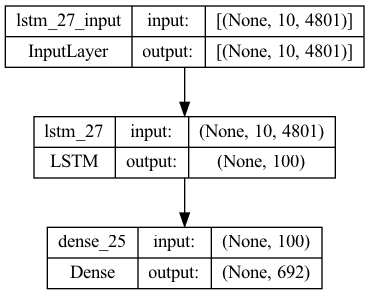
\includegraphics[scale=0.5]{images/model_plot.png}
%     \caption{An example LSTM Network with Input, LSTM and Dense Layer with 4801 Features and window\_size of 10.}
%     \label{fig:lstm_architecture}
% \end{figure}

%\noindent
